\chapter{QuickStart}\label{sec:firstUse}

A Matlab wrapper is delivered with the FA$\mu$ST C++ library.
It provides a user friendly new class of matrix \textbf{FA$\mu$ST} efficient for the multiplication with Matlab built-in dense matrix class.\newline
This chapter presents some demos in order to get a customed to the \textbf{FA$\mu$ST} class and illustrates the advantages of \textbf{FA$\mu$ST} class.  
\begin{enumerate}  
	\item \textbf{Configure your Matlab path} (refer to Section \ref{sec:firstUseMatlabPath}).
	\item You can run and take a look at various Matlab demos :
	\begin{itemize}
		\item \textbf{Use a FA$\mu$ST from a saved one} presents the general functionality of a FA$\mu$ST (go to Section \ref{sec:firstUseBuildFromSave})
		\item \textbf{Construct a FA$\mu$ST from its factor}  (go to  Section \ref{sec:firstUseBuildFactors})
		\item \textbf{Brain Sources Localization}  illustrates the speed-up induced by FA$\mu$ST in a medical application (go to Section \ref{sec:BSL_example})	
	\end{itemize}
\end{enumerate} 





\section{Configure Matlab path}\label{sec:firstUseMatlabPath}
In order to use Matlab wrapper, follow the instructions :

\begin{enumerate}
	\item \textbf{Install} FA$\mu$ST tool (see Chapter \ref{sec:InstallUnix} in case of Unix install or Chapter \ref{sec:WinInstall} in case of Windows install)
	\item \textbf{Launch} Matlab.
	\item \textbf{Set the working directory} of the Matlab Command Window to your FA$\mu$ST install directory FAuST\_INSTALL\_DIR by typing :
		      	\begin{lstlisting}[style=customMatlab]
>> cd <INSTALL_FAuST_DIR>\end{lstlisting}	
	By default, FAuST\_INSTALL\_DIR is inside the Matlab user directory. So, depending on your OS, you must replace the FAuST\_INSTALL\_DIR by this path :
		\begin{itemize} 
			\item \textbf{Windows$\ \ \ $:} \texttt{<ROOT>\textbackslash Users\textbackslash <USERNAME>\textbackslash Documents\textbackslash MATLAB\textbackslash faust}
			\item \textbf{Linux$\ \ \ \ \ \ \ \ $:} \texttt{/home/<USERNAME>/Documents/MATLAB/faust}
			\item \textbf{Mac OS X$\ $:} \texttt{/Users/<USERNAME>/Documents/MATLAB/faust}
		\end{itemize}
	You can also configure the FAuST\_INSTALL\_DIR to whatever you like (cf. CMake variable CMAKE\_INSTALL\_MATLAB\_PREFIX section 		\ref{sec:UnixCustomInstall} for Unix or section \ref{sec:WinCustomInstall} for Windows users)
	



	\item \textbf{Configure} the Matlab path by typing the following commands :
	\lstset{style=customMatlab}
	\begin{lstlisting}
>> setup_Faust \end{lstlisting}
	You must obtain the following message in your Matlab Command Window : 
	\begin{lstlisting}
Welcome to wrapper matlab C++ FAuST_toolbox. 
FAuST root directory is FAuST_INSTALL_DIR
Adding path FAuST_INSTALL_DIR and all its subdirectories 
To get started with the FAuST Toolbox : launch quick_start 
or run_all_demo.m \end{lstlisting}

\end{enumerate}




\section{Use a FAuST from a saved one}\label{sec:firstUseBuildFromSave}
Now, you can run \texttt{quick\_start.m} script in the Matlab Command Window by typing :
\lstset{style=customMatlab}
\begin{lstlisting}
>> quick_start
\end{lstlisting}
\texttt{quick\_start.m} script is located in following path :\\
\texttt{/<INSTALL\_FAuST\_DIR>/demo/Quick\_start/quick\_start.m} \\
In this script :
\begin{enumerate} 
	\item A FA$\mu$ST of size 4000x5000 is loaded from a previous one that is saved into a MAT-file located in :\\
	\texttt{<INSTALL\_FAuST\_DIR>/demo/Quick\_start/faust\_quick\_start.mat}
	\lstinputlisting[firstline=47,lastline=48,style=customMatlab]{../../misc/demo/Quick_start/quick_start.m}
	
	\item  A list of overloaded Matlab function shows that a FA$\mu$ST is handled as a normal Matlab builtin matrix.
 	\lstinputlisting[firstline=51,lastline=83,style=customMatlab]{../../misc/demo/Quick_start/quick_start.m}

	\item It performs a little time comparison between multiplication by a FA$\mu$ST or its full matrix equivalent.
This is in order to illustrate the speed-up induced by the FA$\mu$ST. This speed-up should be around 30 (depending on your machine).
	\lstinputlisting[firstline=88,lastline=104,style=customMatlab]{../../misc/demo/Quick_start/quick_start.m}
\end{enumerate}


\section{Construct a FAuST from its factor}\label{sec:firstUseBuildFactors}
To see an example of building a FA$\mu$ST from its factors, you can run construct\_Faust\_from\_factors.m in the Matlab Command Window by typing :
\lstset{style=customMatlab}
\begin{lstlisting}
>> construct_Faust_from_factors
\end{lstlisting}
This following example shows how to build a FA$\mu$ST from a cell-array representing its factors.
\lstinputlisting[firstline=42,lastline=70,style=customMatlab]{../../misc/demo/Quick_start/construct_Faust_from_factors.m}

If you want to build a FA$\mu$ST from a given matrix, you can go to the section Working Progress \ref{sec:WorkingProgressBuildFromMatrix}.
Be aware that this not yet stable but under progress.



\section{Brain Sources Localization}\label{sec:BSL_example}
%\lstinputlisting{../../misc/demo/Brain_source_localization/BSL.m}
An experience of Brain Source Localization using several gain matrices including FA$\mu$ST and several solvers is provided. After configuring the Matlab path (cf. section \ref{sec:firstUseMatlabPath}), you just need to type in the Matlab Command Window:

\lstset{style=customMatlab}
\begin{lstlisting}
>> BSL
>> Fig_BSL
\end{lstlisting}

\texttt{BSL.m} runs the experiment (see the script file :\\
\texttt{/<FAuST\_INSTALL\_DIR>/demo/Brain\_source\_localization/BSL.m})\\
\texttt{Fig\_BSL.m} displays the Figure \ref{fig:BSL}. illustrating the speed-up using a FA$\mu$ST. (see the script file:\\
\texttt{<FAuST\_INSTALL\_DIR>/demo/Brain\_source\_localization/Fig\_BSL.m}) \\

This figure illustrates the speed-up with a FA$\mu$ST ($\mathbf{M}$ is the gain dense matrix and $\widehat{\mathbf{M}}_{6},\widehat{\mathbf{M}}_{9},\widehat{\mathbf{M}}_{16},\widehat{\mathbf{M}}_{26}$ are different FA$\mu$ST representing  $\mathbf{M}$):


\begin{figure}[H] %%[!htbp]
\centering
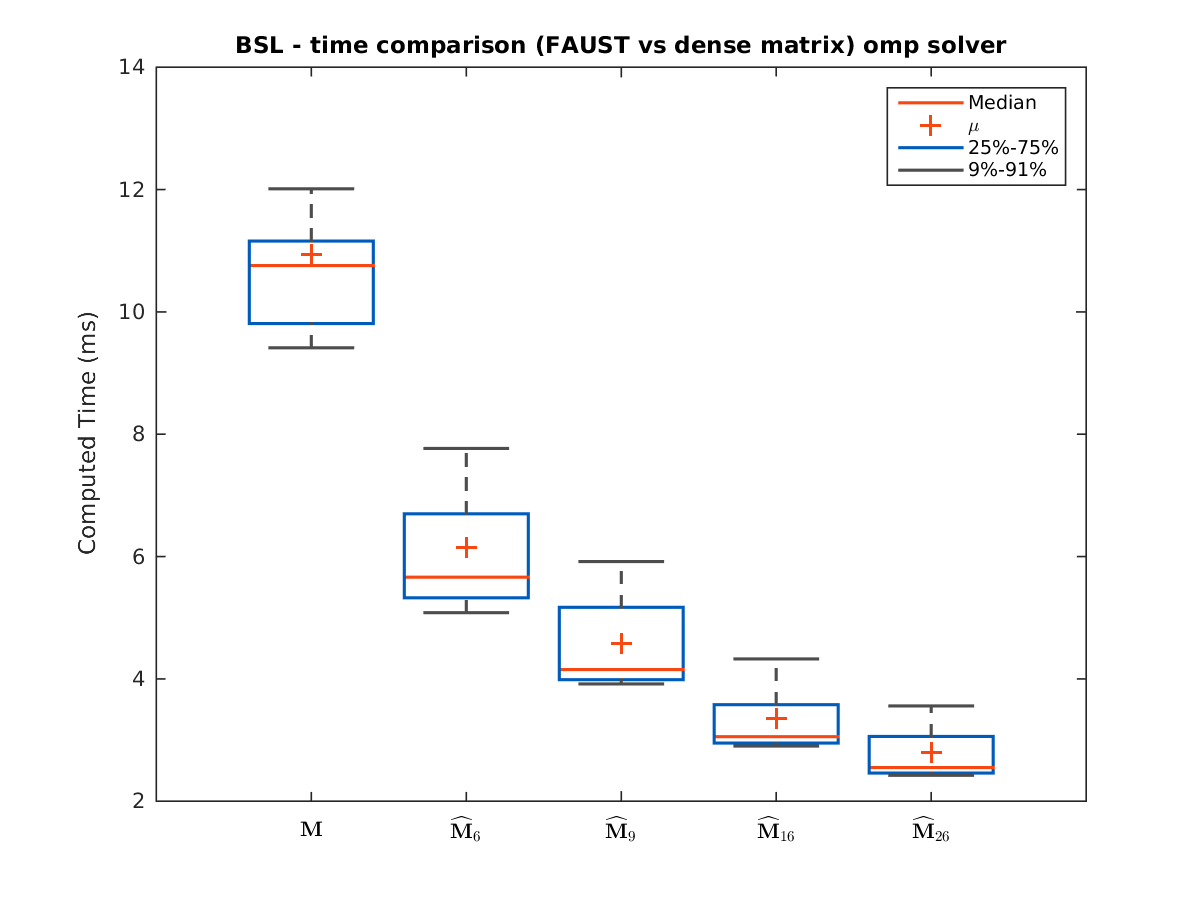
\includegraphics[scale=0.7]{images/BSL.png}
\caption{Performance of FA$\mu$ST tool on Brain Source Localization experiment}
\label{fig:BSL}
\end{figure}






 
